\documentclass{article}
\usepackage{amsmath}
\usepackage{amssymb}
\usepackage{graphicx}
\usepackage{hyperref}
\usepackage[version=4]{mhchem}

\title{Example 9}
\date{}

\begin{document}
\maketitle

As shown in the figure below, in square \(A B C D, F\) is the midpoint of \(D C\). \(E\) is a point on \(B C\) such that \(A E=D C+C E\). Show that \(A F\) bisects \(\angle D A E\).

Solution:
Method 1:\\
\centering
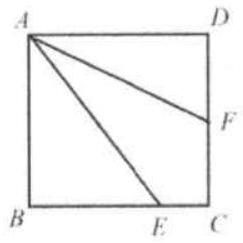
\includegraphics[width=\textwidth]{images/060.jpg}

Connect \(E F\) and extend it to meet the extension of \(A D\) at \(G\). look at triangles \(F D G\) and \(F C E\).\\
We see that \(F D=F C, \angle D F G=\angle C F E, \angle C=\angle F D G\).\\
Thus, \(\triangle F D G \cong \triangle F C E\) and \(D G=C E, E F=F G\).\\
So \(A G=A D+D G=D C+C E=A E\).\\
Since \(E F=F G, A E=A G, A F=A F, \triangle A F G \cong \triangle A F E\).\\
\centering
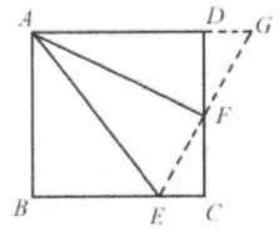
\includegraphics[width=\textwidth]{images/060(1).jpg}

Therefore, \(\angle E A F=\angle G A F, A F\) bisects \(\angle D A E\).\\
Method 2:\\
Extend \(A F\) to meet the extension of \(B C\) at \(G\).\\
Connect \(E F\). Triangles \(A D F\) and \(G D F\) are congruent.\\
\centering
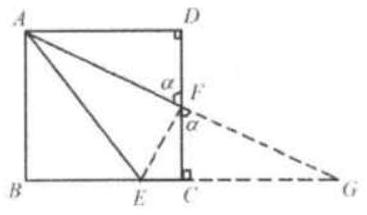
\includegraphics[width=\textwidth]{images/060(2).jpg}

So \(A D=C G . \angle D A F=\angle C G F\).\\
\(A E=D C+C E=G C+C E=G E\).

So triangle \(A E G\) is an isosceles triangle with \(A E=G E\) or \(\angle E A F=\angle G G F\).\\
So \(\angle D A F=\angle E A F\). \(A F\) bisects \(\angle D A E\).


\end{document}
